\section{KStartup\-Logo Class Reference}
\label{classKStartupLogo}\index{KStartupLogo@{KStartupLogo}}
{\tt \#include $<$kstartuplogo.h$>$}

Inheritance diagram for KStartup\-Logo:\begin{figure}[H]
\begin{center}
\leavevmode
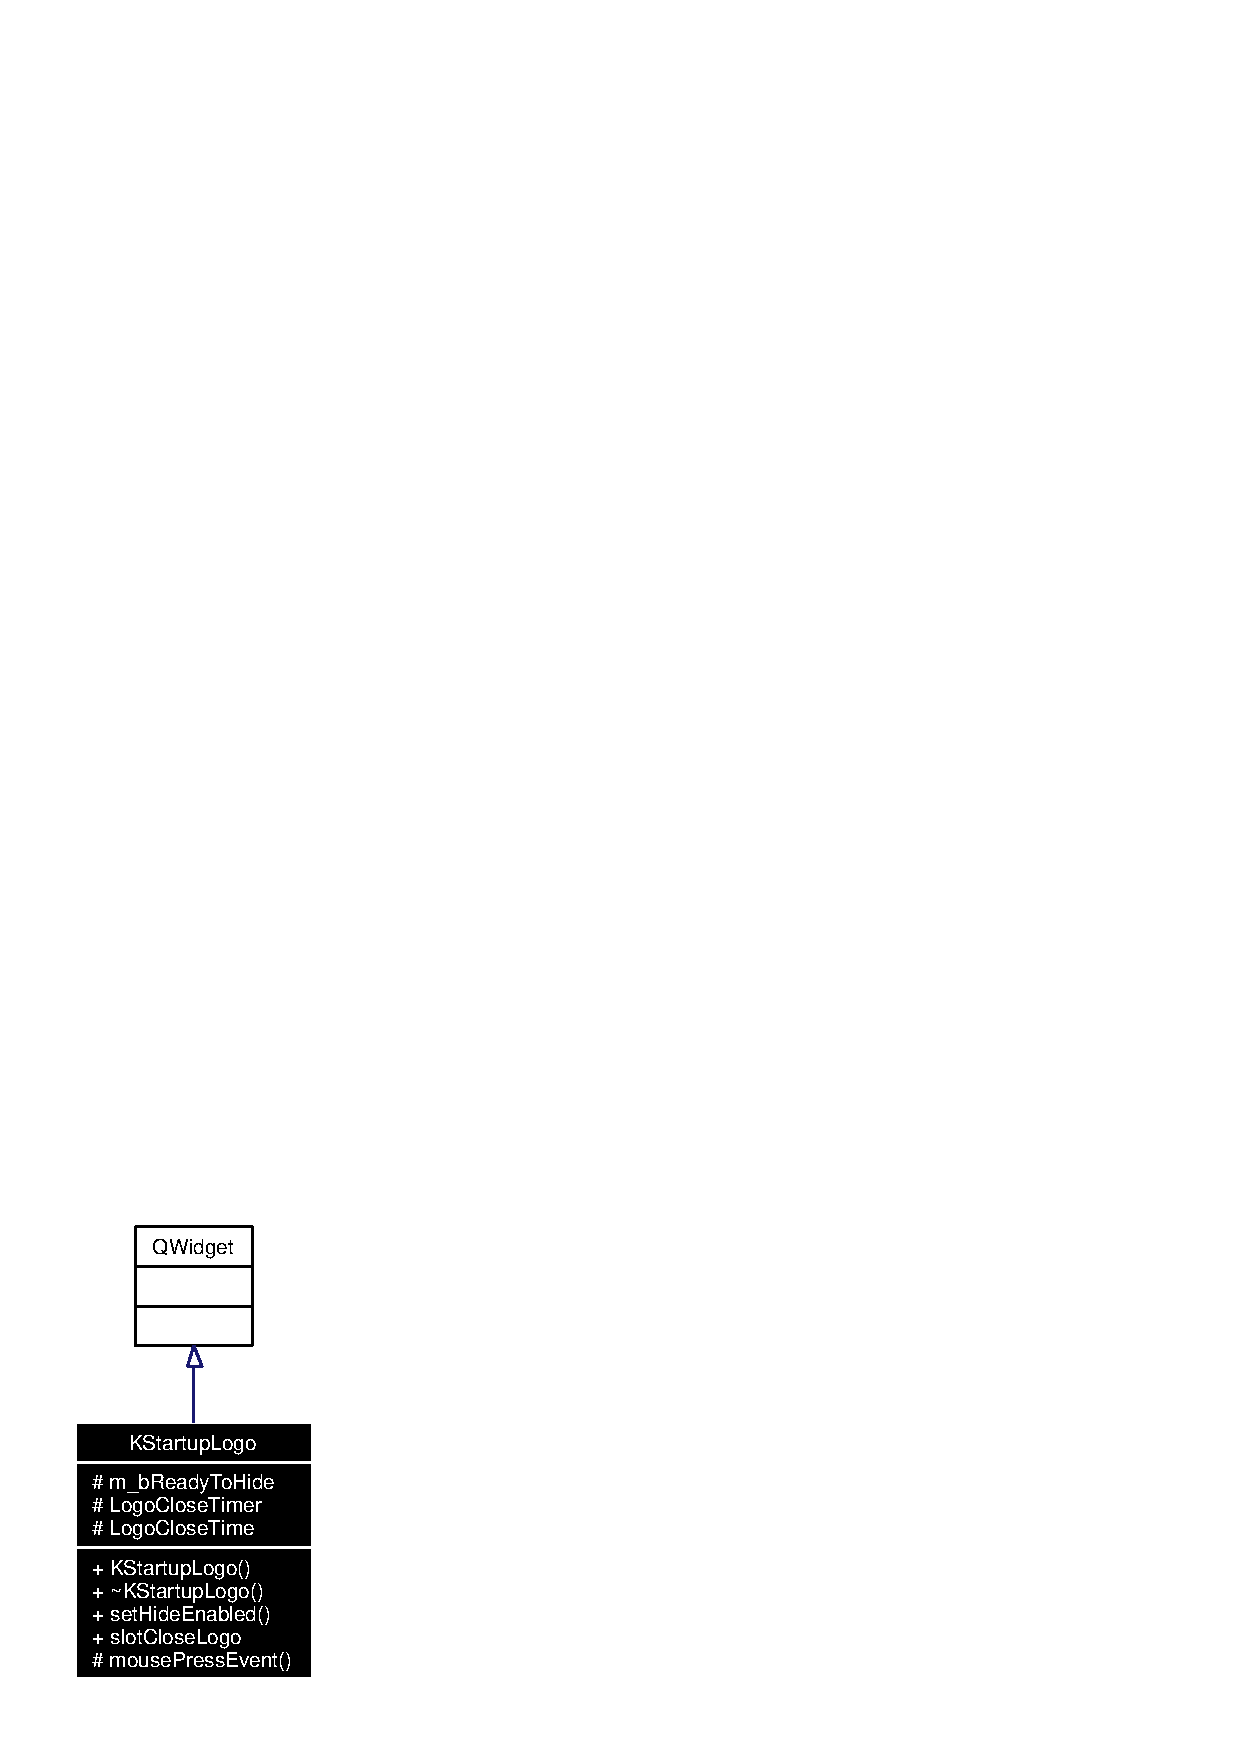
\includegraphics[width=75pt]{classKStartupLogo__inherit__graph}
\end{center}
\end{figure}
Collaboration diagram for KStartup\-Logo:\begin{figure}[H]
\begin{center}
\leavevmode
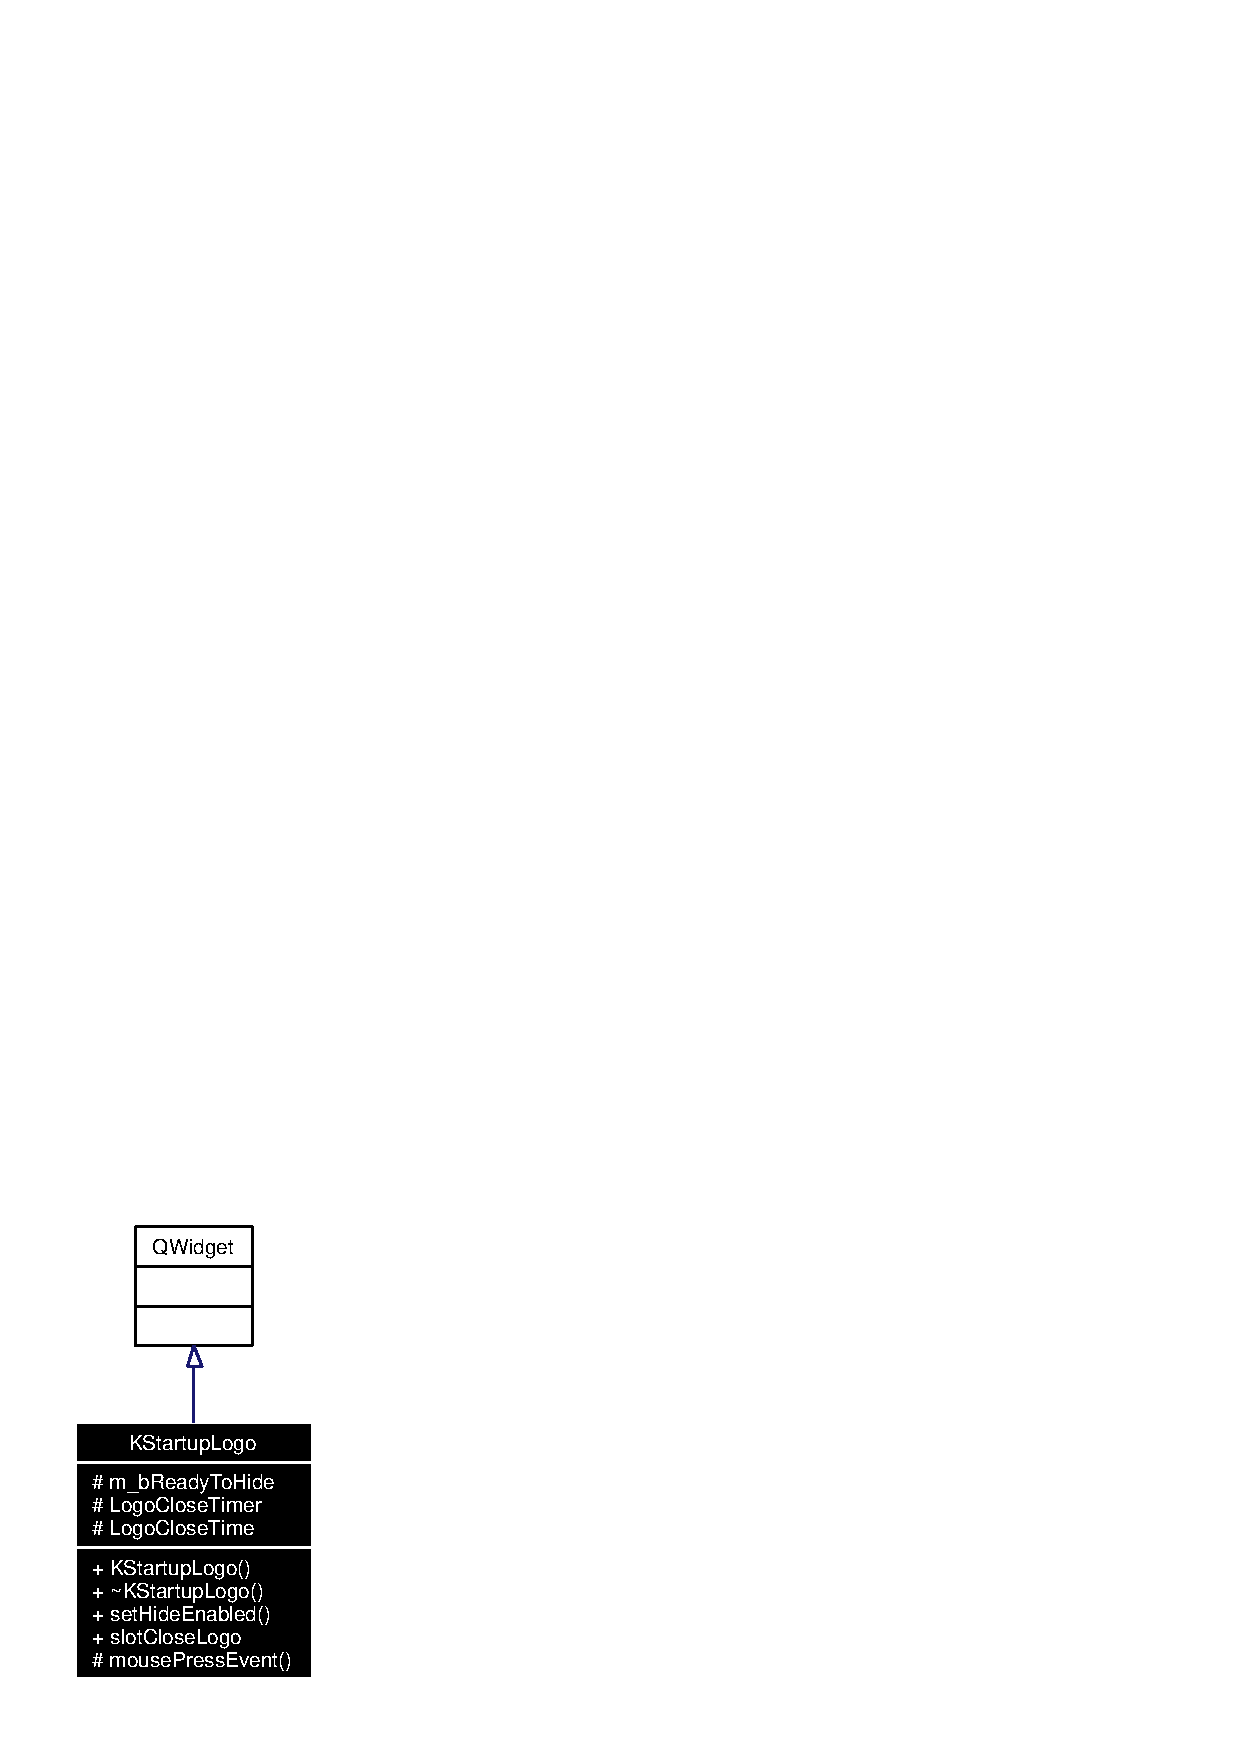
\includegraphics[width=75pt]{classKStartupLogo__coll__graph}
\end{center}
\end{figure}


\subsection{Detailed Description}
\begin{Desc}
\item[Author:]\end{Desc}




Definition at line 31 of file kstartuplogo.h.\subsection*{Public Slots}
\begin{CompactItemize}
\item 
void {\bf slot\-Close\-Logo} ()
\end{CompactItemize}
\subsection*{Signals}
\begin{CompactItemize}
\item 
void {\bf signal\-Trigger\-Main\-Widget} ()
\end{CompactItemize}
\subsection*{Public Member Functions}
\begin{CompactItemize}
\item 
{\bf KStartup\-Logo} ({\bf QWidget} $\ast$parent=0, const char $\ast$name=0)
\item 
{\bf $\sim$KStartup\-Logo} ()
\item 
void {\bf set\-Hide\-Enabled} (bool b\-Enabled)
\end{CompactItemize}
\subsection*{Protected Member Functions}
\begin{CompactItemize}
\item 
virtual void {\bf mouse\-Press\-Event} (QMouse\-Event $\ast$)
\end{CompactItemize}
\subsection*{Protected Attributes}
\begin{CompactItemize}
\item 
bool {\bf m\_\-b\-Ready\-To\-Hide}
\item 
QTimer $\ast$ {\bf Logo\-Close\-Timer}
\item 
int {\bf Logo\-Close\-Time}
\end{CompactItemize}


\subsection{Constructor \& Destructor Documentation}
\index{KStartupLogo@{KStartup\-Logo}!KStartupLogo@{KStartupLogo}}
\index{KStartupLogo@{KStartupLogo}!KStartupLogo@{KStartup\-Logo}}
\subsubsection{\setlength{\rightskip}{0pt plus 5cm}KStartup\-Logo::KStartup\-Logo ({\bf QWidget} $\ast$ {\em parent} = 0, const char $\ast$ {\em name} = 0)}\label{classKStartupLogo_KStartupLogoa0}




Definition at line 23 of file kstartuplogo.cpp.

References Logo\-Close\-Time, Logo\-Close\-Timer, and slot\-Close\-Logo().



\footnotesize\begin{verbatim}23                                                              : QWidget(parent,name, WStyle_NoBorder | WStyle_Customize | WDestructiveClose ), m_bReadyToHide( false ),LogoCloseTimer(NULL),LogoCloseTime(1){
24         QPixmap pm;
25         pm.load("/root/kde_application/hdass08/skin/skin-logo.jpg");
26         setBackgroundPixmap(pm);
27         setGeometry(KApplication::desktop()->width()/2-pm.width()/2, KApplication::desktop()->height()/2-pm.height()/2, pm.width(),pm.height());
28         
29         //DAVID Timer Set up
30         LogoCloseTimer=new QTimer(this);
31         //DAVID Connect LogoCloseTimer to slot "slotCloseLogo"
32         connect(LogoCloseTimer,SIGNAL(timeout()),this,SLOT(slotCloseLogo()));
33         LogoCloseTimer->start( LogoCloseTime*1000, TRUE ); // 2 seconds single-shot timer
34 }
\end{verbatim}\normalsize 
\index{KStartupLogo@{KStartup\-Logo}!~KStartupLogo@{$\sim$KStartupLogo}}
\index{~KStartupLogo@{$\sim$KStartupLogo}!KStartupLogo@{KStartup\-Logo}}
\subsubsection{\setlength{\rightskip}{0pt plus 5cm}KStartup\-Logo::$\sim${\bf KStartup\-Logo} ()}\label{classKStartupLogo_KStartupLogoa1}




Definition at line 36 of file kstartuplogo.cpp.



\footnotesize\begin{verbatim}37 {
38 }
\end{verbatim}\normalsize 


\subsection{Member Function Documentation}
\index{KStartupLogo@{KStartup\-Logo}!mousePressEvent@{mousePressEvent}}
\index{mousePressEvent@{mousePressEvent}!KStartupLogo@{KStartup\-Logo}}
\subsubsection{\setlength{\rightskip}{0pt plus 5cm}void KStartup\-Logo::mouse\-Press\-Event (QMouse\-Event $\ast$)\hspace{0.3cm}{\tt  [protected, virtual]}}\label{classKStartupLogo_KStartupLogob0}




Definition at line 40 of file kstartuplogo.cpp.

References m\_\-b\-Ready\-To\-Hide.



\footnotesize\begin{verbatim}41 {
42         if (m_bReadyToHide) hide();
43 }
\end{verbatim}\normalsize 
\index{KStartupLogo@{KStartup\-Logo}!setHideEnabled@{setHideEnabled}}
\index{setHideEnabled@{setHideEnabled}!KStartupLogo@{KStartup\-Logo}}
\subsubsection{\setlength{\rightskip}{0pt plus 5cm}void KStartup\-Logo::set\-Hide\-Enabled (bool {\em b\-Enabled})\hspace{0.3cm}{\tt  [inline]}}\label{classKStartupLogo_KStartupLogoa2}




Definition at line 38 of file kstartuplogo.h.

References m\_\-b\-Ready\-To\-Hide.



\footnotesize\begin{verbatim}38 { m_bReadyToHide = bEnabled; };
\end{verbatim}\normalsize 
\index{KStartupLogo@{KStartup\-Logo}!signalTriggerMainWidget@{signalTriggerMainWidget}}
\index{signalTriggerMainWidget@{signalTriggerMainWidget}!KStartupLogo@{KStartup\-Logo}}
\subsubsection{\setlength{\rightskip}{0pt plus 5cm}void KStartup\-Logo::signal\-Trigger\-Main\-Widget ()\hspace{0.3cm}{\tt  [signal]}}\label{classKStartupLogo_KStartupLogol0}




Definition at line 84 of file kstartuplogo.moc.

Referenced by slot\-Close\-Logo().



\footnotesize\begin{verbatim}85 {
86     activate_signal( staticMetaObject()->signalOffset() + 0 );
87 }
\end{verbatim}\normalsize 
\index{KStartupLogo@{KStartup\-Logo}!slotCloseLogo@{slotCloseLogo}}
\index{slotCloseLogo@{slotCloseLogo}!KStartupLogo@{KStartup\-Logo}}
\subsubsection{\setlength{\rightskip}{0pt plus 5cm}void KStartup\-Logo::slot\-Close\-Logo ()\hspace{0.3cm}{\tt  [slot]}}\label{classKStartupLogo_KStartupLogoi0}




Definition at line 45 of file kstartuplogo.cpp.

References signal\-Trigger\-Main\-Widget().

Referenced by KStartup\-Logo().



\footnotesize\begin{verbatim}46 {
47    //DAVID Hide Logo itself.
48    this->hide();
49    emit signalTriggerMainWidget();
50 }
\end{verbatim}\normalsize 


\subsection{Member Data Documentation}
\index{KStartupLogo@{KStartup\-Logo}!LogoCloseTime@{LogoCloseTime}}
\index{LogoCloseTime@{LogoCloseTime}!KStartupLogo@{KStartup\-Logo}}
\subsubsection{\setlength{\rightskip}{0pt plus 5cm}int {\bf KStartup\-Logo::Logo\-Close\-Time}\hspace{0.3cm}{\tt  [protected]}}\label{classKStartupLogo_KStartupLogop2}




Definition at line 47 of file kstartuplogo.h.

Referenced by KStartup\-Logo().\index{KStartupLogo@{KStartup\-Logo}!LogoCloseTimer@{LogoCloseTimer}}
\index{LogoCloseTimer@{LogoCloseTimer}!KStartupLogo@{KStartup\-Logo}}
\subsubsection{\setlength{\rightskip}{0pt plus 5cm}QTimer$\ast$ {\bf KStartup\-Logo::Logo\-Close\-Timer}\hspace{0.3cm}{\tt  [protected]}}\label{classKStartupLogo_KStartupLogop1}




Definition at line 46 of file kstartuplogo.h.

Referenced by KStartup\-Logo().\index{KStartupLogo@{KStartup\-Logo}!m_bReadyToHide@{m\_\-bReadyToHide}}
\index{m_bReadyToHide@{m\_\-bReadyToHide}!KStartupLogo@{KStartup\-Logo}}
\subsubsection{\setlength{\rightskip}{0pt plus 5cm}bool {\bf KStartup\-Logo::m\_\-b\-Ready\-To\-Hide}\hspace{0.3cm}{\tt  [protected]}}\label{classKStartupLogo_KStartupLogop0}




Definition at line 45 of file kstartuplogo.h.

Referenced by mouse\-Press\-Event(), and set\-Hide\-Enabled().

The documentation for this class was generated from the following files:\begin{CompactItemize}
\item 
{\bf kstartuplogo.h}\item 
{\bf kstartuplogo.moc}\item 
{\bf kstartuplogo.cpp}\end{CompactItemize}
